\chapter{Spektroskopi Rotasi dan Vibrasi}\label{ch:b3:rovibrational-spectroscopy}

Di sebuah dataran tinggi yang kering, puluhan antena radio mengarah ke
sebuah awan gelap di antara bintang-bintang. Di antara frekuensi-frekuensi
yang dikumpulkannya terdapat satu frekuensi pada \qty{115.271}{GHz}:
molekul-molekul karbon monoksida, pada suhu beberapa kelvin, yang berpindah
dari tingkat rotasi pertamanya ke tingkat terendah. Dari satu angka itu saja
seorang kimiawan memperoleh panjang ikatan C--O sampai sepersekian pikometer;
dari kuat garis-garis berikutnya, suhu awan itu. Rotasi dan vibrasi molekul
adalah pokok bahasan bab ini: tingkat-tingkat energinya, dari rotor dan
osilator \cref{ch:b3:quantum-model-systems}; aturan seleksinya, dari
\cref{ch:b3:group-theory-applied}; dan apa yang diukur oleh spektrum ---
panjang ikatan, \omterm{def:b3:quantum-model-systems:oscillator}{tetapan gaya}, energi disosiasi.

\begin{recall}
\Cref{ch:b3:quantum-model-systems} memberikan \omterm{def:b3:quantum-model-systems:rotor}{rotor tegar},
$E_J = J(J+1)\hbar^2/2I$ dengan \omterm{def:b3:quantum-model-systems:degenerate}{degenerasi} $2J + 1$, dan \omterm{def:b3:quantum-model-systems:oscillator}{osilator harmonik},
$E_v = (v + \frac12)h\nu$, untuk molekul diatomik dengan \omterm{def:b3:quantum-model-systems:oscillator}{massa tereduksi} $\mu$.
\Cref{ch:b3:group-theory-applied} menyatakan aturan seleksi inframerah dan
Raman. Jilid Tahun 1 mengukur spektrum inframerah dalam bilangan gelombang dan
mendefinisikan polarisabilitas sebuah molekul.
\end{recall}

\begin{omfigure}
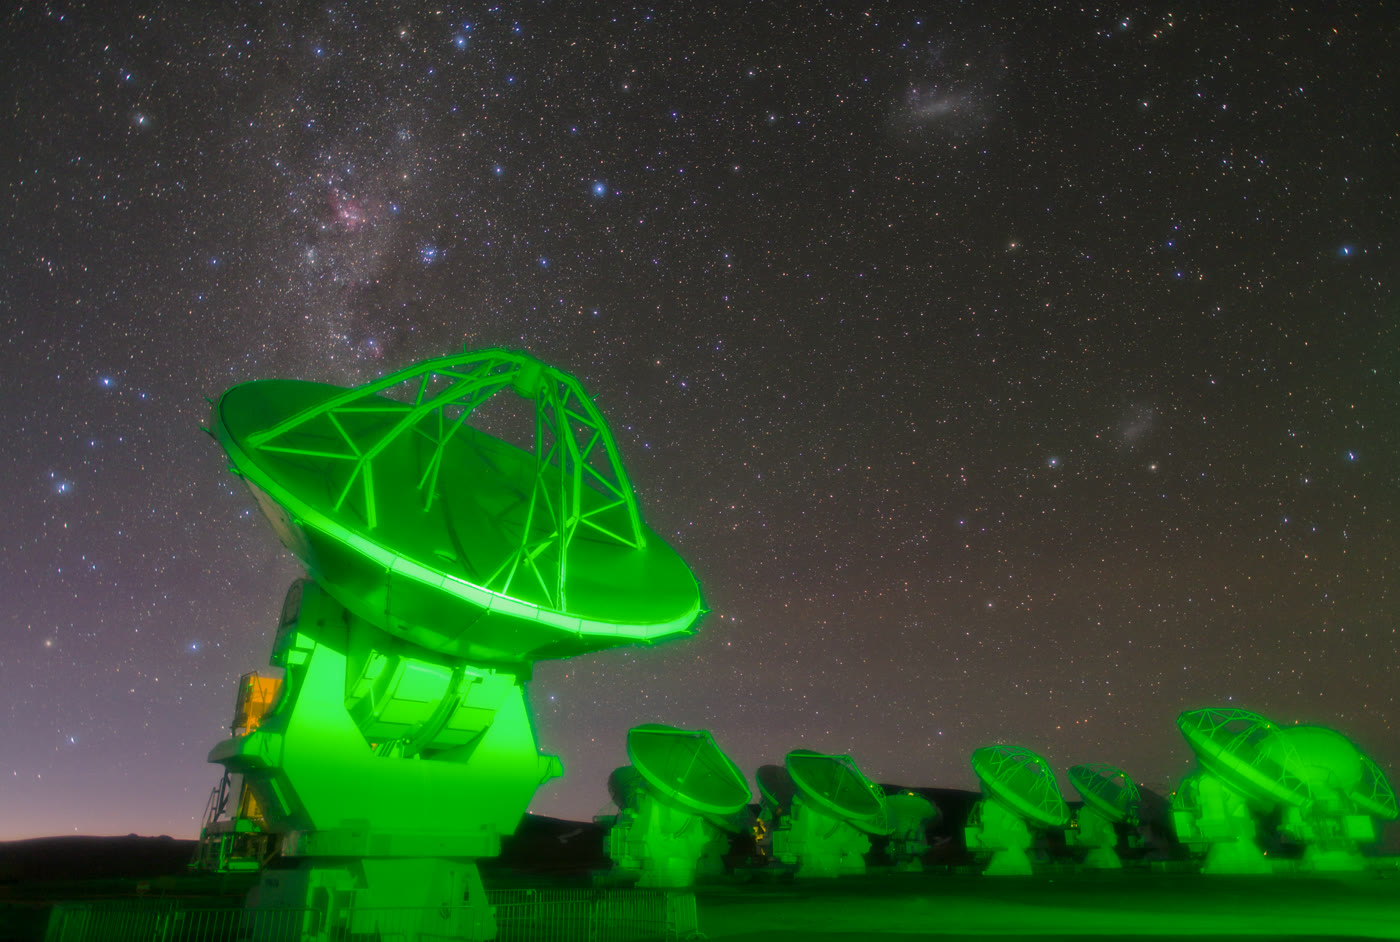
\includegraphics[width=0.7\linewidth]{images/book4/alma-antennas.jpg}

{\small Antena-antena sebuah interferometer radio di sebuah dataran tinggi:
antena-antena itu merekam, di antara banyak garis lain, garis-garis rotasi
karbon monoksida dari awan antarbintang. Foto ESO/B.~Tafreshi (twanight.org),
CC\ BY\ 4.0.}
\end{omfigure}

\section{Spektrum rotasi}

\begin{definition}[Tetapan rotasi, isotopolog]\label{def:b3:rovibrational-spectroscopy:rotational-constant}
Yang disebut \emph{tetapan rotasi}\index{tetapan rotasi} molekul linear adalah
$B = h/(8\pi^2cI)$, dalam \unit{cm^{-1}} (atau $B = h/8\pi^2I$ dalam hertz),
sehingga tingkat-tingkat rotasinya adalah $F(J) = BJ(J+1)$ dalam bilangan
gelombang. Molekul-molekul yang hanya berbeda pada isotop atom-atomnya
disebut \emph{isotopolog}\index{isotopolog} (\ce{^{12}C^{16}O}, \ce{^{13}C^{16}O});
dalam \omterm{def:b3:computational-chemistry:born-oppenheimer}{pendekatan Born--Oppenheimer}, isotopolog-isotopolog itu mempunyai
panjang ikatan dan \omterm{def:b3:quantum-model-systems:oscillator}{tetapan gaya} yang sama.
\end{definition}

\begin{definition}[Aturan seleksi umum dan khusus]\label{def:b3:rovibrational-spectroscopy:selection}
Yang disebut \emph{aturan seleksi umum}\index{aturan seleksi umum} adalah
aturan yang menyatakan sifat apa yang harus dimiliki sebuah molekul agar
memperlihatkan suatu jenis spektrum sama sekali; yang disebut \emph{aturan
seleksi khusus}\index{aturan seleksi khusus} adalah aturan yang menyatakan
perubahan bilangan kuantum mana yang diizinkan.
\end{definition}

\begin{proposition}[Spektrum rotasi murni]\label{prop:b3:rovibrational-spectroscopy:rotational-lines}
Sebuah molekul hanya mempunyai spektrum rotasi murni (gelombang mikro) jika
molekul itu mempunyai momen dipol permanen; untuk molekul linear, aturan
khususnya adalah $\Delta J
= \pm1$. Garis-garis serapannya terletak pada
\[
\tilde\nu = F(J+1) - F(J) = 2B(J + 1), \qquad J = 0, 1, 2, \dots,
\]
yang berjarak sama sebesar $2B$.
\end{proposition}

\begin{proof}
Interaksi dengan cahaya berlangsung melalui momen dipol: molekul tanpa dipol
permanen tidak mempunyai dipol yang berosilasi ketika berputar. Aturan
$\Delta J
= \pm1$ berasal dari lenyapnya $\int Y_{J'M'}^*\cos\theta\,Y_{JM}$ kecuali
jika $J' = J
\pm 1$ (komponen dipol sepanjang $z$ bertransformasi seperti
$Y_{1,0}$), yang diterima tanpa bukti. Lalu $B(J+1)(J+2) - BJ(J+1) = 2B(J+1)$.
\end{proof}

\begin{method}[Panjang ikatan dari sebuah garis rotasi]\label{met:b3:rovibrational-spectroscopy:bond-length}
\begin{enumerate}
  \item Dari garis $J + 1 \leftarrow J$ pada frekuensi $\nu$, simpulkan
        $B =
        \nu/2(J+1)$ (dalam hertz).
  \item Hitunglah momen inersia $I = h/8\pi^2B$.
  \item Dengan \omterm{def:b3:quantum-model-systems:oscillator}{massa tereduksi} dari massa-massa isotop, $r = \sqrt{I/\mu}$.
\end{enumerate}
\end{method}

\begin{example}[Karbon monoksida]\label{ex:b3:rovibrational-spectroscopy:co}
% ledger: rotl:CO.1-0, imass:O16
Garis $J = 1 \leftarrow 0$ dari \ce{^{12}C^{16}O} terletak pada
\qty{115271.20}{MHz}: $B = \qty{57635.6}{MHz} = \qty{1.92252}{cm^{-1}}$,
$I = \qty{1.4560e-46}{kg.m^2}$. Dengan $\mu = 12 \times 15.99491/27.99491 = \qty{6.85621}{u}$,
$r_0 = \qty{113.09}{pm}$. Nilai $r_0$ ini merata-ratakan ikatan atas vibrasi
titik nolnya dan sedikit lebih panjang daripada panjang kesetimbangan $r_e$
(\cref{sec:b3:rovibrational-spectroscopy:real-bonds}).
\end{example}

\begin{definition}[Tetapan distorsi sentrifugal]\label{def:b3:rovibrational-spectroscopy:centrifugal}
Ikatan yang berputar akan meregang; tingkat-tingkat energinya menjadi
$F(J) = BJ(J+1) - DJ^2(J+1)^2$, dengan $D$ yang disebut \emph{tetapan distorsi
sentrifugal}\index{tetapan distorsi sentrifugal}, dan garis-garis
$2B(J+1) - 4D(J+1)^3$ perlahan-lahan merapat pada $J$ yang tinggi.
\end{definition}

\begin{proposition}[Garis terkuat]\label{prop:b3:rovibrational-spectroscopy:jmax}
Jika intensitas garis mengikuti populasi tingkat bawah, $(2J+1)
\eu^{-hcBJ(J+1)/kT}$, tingkat yang paling terpopulasi berada di dekat
\[
J_{\max} \approx \sqrt{\frac{kT}{2hcB}} - \frac12.
\]
\end{proposition}

\begin{proof}
Perlakukan $J$ sebagai kontinu lalu turunkan: $\frac{\dd}{\dd J}[(2J+1)\eu^{-aJ(J+1)}]
= [2 - a(2J+1)^2]\eu^{-aJ(J+1)}$ dengan $a = hcB/kT$; turunan itu lenyap pada
$(2J + 1)^2 =
2/a$.
\end{proof}

\begin{omfigure}
\begin{tikzpicture}
\begin{axis}[width=0.9\linewidth, height=4.8cm, xmin=0, xmax=70, ymin=0,
  ymax=1.12, ytick=\empty, axis x line=bottom, axis y line=left, ycomb,
  xlabel={bilangan gelombang / cm$^{-1}$}, ylabel={intensitas relatif},
  tick label style={font=\small}, label style={font=\small}]
\addplot[omDef, very thick] table[x=nu, y=I] {figdata/out/bachelor-3-rotational-spectrum-co-30.dat};
\addplot[omThm, thick, xshift=1.2pt] table[x=nu, y=I] {figdata/out/bachelor-3-rotational-spectrum-co-300.dat};
\end{axis}
\end{tikzpicture}

{\small Spektrum serapan rotasi karbon monoksida, dengan garis-garis berjarak
$2B = \qty{3.845}{cm^{-1}}$ dan intensitas yang diambil sebagai populasi
tingkat bawah, pada \qty{30}{K} (biru) dan \qty{300}{K} (merah, sedikit
digeser agar terlihat), setiap suhu diskalakan terhadap garis terkuatnya. Pada
\qty{30}{K} garis terkuat adalah $J = 3 \leftarrow 2$; pada \qty{300}{K},
$J = 8 \leftarrow 7$.}
\end{omfigure}

\section{Vibrasi ikatan nyata}\label{sec:b3:rovibrational-spectroscopy:real-bonds}

Ikatan yang nyata tidak mematuhi hukum Hooke jauh dari kesetimbangan: ikatan
itu melunak ketika diregangkan, lalu putus.

\begin{definition}[Potensial Morse]\label{def:b3:rovibrational-spectroscopy:morse}
Yang disebut \emph{potensial Morse}\index{potensial Morse} adalah $V(r) = D_e[1 -
\eu^{-\beta(r - r_e)}]^2$: harmonik di dekat $r_e$ (\omterm{def:b3:quantum-model-systems:oscillator}{tetapan gaya} $2\beta^2D_e$),
dan menuju batas disosiasi $D_e$ pada $r$ yang besar.
\end{definition}

\begin{proposition}[Tingkat energi osilator Morse]\label{prop:b3:rovibrational-spectroscopy:morse-levels}
Dalam bilangan gelombang, tingkat-tingkat vibrasi osilator Morse adalah
\[
G(v) = \tilde\omega_e(v + \tfrac12) - \tilde\omega_ex_e(v + \tfrac12)^2, \qquad
\tilde\omega_ex_e = \frac{\tilde\omega_e^2}{4D_e},
\]
sebuah tangga yang anak tangganya makin merapat dan berakhir pada
$v_{\max} = \lfloor\tilde\omega_e/
2\tilde\omega_ex_e - \frac12\rfloor$.
\end{proposition}
\admitted

Penyelesaian persamaan Morse dibahas dalam kuliah yang lebih lanjut;
tingkat-tingkat energinya diperiksa secara numerik dalam data gambar bab ini.

\begin{definition}[Tetapan anharmonisitas, fundamental, overtone, pita panas]\label{def:b3:rovibrational-spectroscopy:anharmonic}
$\tilde\omega_ex_e$ adalah \emph{tetapan anharmonisitas}\index{tetapan anharmonisitas}.
Yang disebut \emph{transisi fundamental}\index{transisi fundamental} adalah
$v = 1 \leftarrow 0$; sebuah \emph{overtone}\index{overtone} adalah
$v = n \leftarrow 0$ dengan $n \ge 2$, yang lemah karena aturan umum
$\Delta v = \pm1$ \omterm{def:b3:quantum-model-systems:oscillator}{osilator harmonik} hanya sedikit dilanggar; sebuah
\emph{pita panas}\index{pita panas} berawal dari tingkat tereksitasi,
$v = 2 \leftarrow 1$, dan menguat bersama suhu.
\end{definition}

\begin{definition}[Energi disosiasi spektroskopis]\label{def:b3:rovibrational-spectroscopy:dissociation}
Yang disebut \emph{energi disosiasi
spektroskopis}\index{energi disosiasi spektroskopis} sebuah molekul adalah kedalaman potensialnya, $D_e$, yang
diukur dari minimum, atau $D_0 = D_e - G(0)$, yang diukur dari tingkat
terendah --- per molekul pada \qty{0}{K}, berbeda dengan entalpi disosiasi
ikatan dalam jilid Tahun 2, yang merupakan entalpi molar pada \qty{298}{K}.
\end{definition}

\begin{corollary}[$D_e$ dan $D_0$ osilator Morse]\label{cor:b3:rovibrational-spectroscopy:de}
$D_e = \tilde\omega_e^2/4\tilde\omega_ex_e$ dan $D_0 = D_e - (\frac12\tilde\omega_e -
\frac14\tilde\omega_ex_e)$.
\end{corollary}

\begin{proof}
Yang pertama adalah hubungan dalam proposisi di atas; yang kedua adalah $G(0)$.
\end{proof}

\begin{proposition}[Ekstrapolasi Birge--Sponer]\label{prop:b3:rovibrational-spectroscopy:birge-sponer}
Selisih-selisih $\Delta G(v + \frac12) = G(v+1) - G(v) = \tilde\omega_e - 2\tilde\omega_ex_e(v +
1)$ mengecil secara linear terhadap $v$; menjumlahkannya sampai selisih itu
lenyap memberikan $D_0$, yaitu luas di bawah grafik $\Delta G$ terhadap $v$.
\end{proposition}

\begin{proof}
Kurangkan kedua ungkapan $G$. $D_0$ adalah energi dari $v = 0$ sampai batas
disosiasi, yaitu jumlah semua selisih itu.
\end{proof}

\begin{example}[Hidrogen klorida]\label{ex:b3:rovibrational-spectroscopy:hcl}
% ledger: diat:HCl.we, diat:HCl.wexe, janaf:H.dfH0, janaf:Cl.dfH0, janaf:HCl.dfH0
Untuk \ce{H^{35}Cl}, $\tilde\omega_e = \qty{2990.95}{cm^{-1}}$ dan
$\tilde\omega_ex_e =
\qty{52.82}{cm^{-1}}$: fundamentalnya terletak pada
$\tilde\omega_e - 2\tilde\omega_ex_e =
\qty{2885.3}{cm^{-1}}$ dan \omterm{def:b3:rovibrational-spectroscopy:anharmonic}{overtone} pertamanya
pada $2\tilde\omega_e - 6\tilde\omega_ex_e =
\qty{5665.0}{cm^{-1}}$, sedikit kurang dari
dua kali fundamental. Model Morse meramalkan $D_e = \qty{42342}{cm^{-1}}$ dan
$D_0 = \qty{40860}{cm^{-1}}$; $D_0$ yang sebenarnya, dari entalpi pembentukan H,
Cl dan HCl pada \qty{0}{K}, adalah \qty{35760}{cm^{-1}} (\qty{4.43}{eV}).
Potensial yang nyata mendatar lebih cepat daripada kurva Morse yang
dicocokkan di bagian dasarnya: ekstrapolasi Birge--Sponer dari tingkat-tingkat
terendah menaksir energi disosiasi terlalu tinggi.
\end{example}

\begin{omfigure}
\begin{tikzpicture}
\begin{axis}[name=morse, width=0.55\linewidth, height=6cm, xmin=0.8, xmax=4.0,
  ymin=0, ymax=48000, axis lines=left, xlabel={$r$ / \AA}, ylabel={$V$ / cm$^{-1}$},
  unbounded coords=jump, scaled y ticks=false, ytick={0,10000,20000,30000,40000},
  tick label style={font=\small}, label style={font=\small}]
\addplot[black, thick] table[x=r, y=V] {figdata/out/bachelor-3-morse-levels.dat};
\addplot[gray, dashed] table[x=r, y=harm] {figdata/out/bachelor-3-morse-levels.dat};
\addplot[omDef] table[x=r, y=E] {figdata/out/bachelor-3-morse-levels-levels.dat};
\draw[<->, omThm] (axis cs:3.7,0) -- (axis cs:3.7,42342) node[pos=0.5, left, font=\small] {$D_e$};
\draw[dashed, omThm] (axis cs:1.2,42342) -- (axis cs:4.0,42342);
\end{axis}
\begin{axis}[at={(morse.east)}, anchor=west, xshift=1.6cm, width=0.4\linewidth,
  height=5cm, xmin=0, xmax=28, ymin=0, ymax=3100, axis lines=left,
  xlabel={$v$}, ylabel={$\Delta G(v + \frac12)$ / cm$^{-1}$},
  tick label style={font=\small}, label style={font=\small}]
\addplot[omDef, only marks, mark size=1.2pt] table[x=v, y=dG] {figdata/out/bachelor-3-morse-levels-bs.dat};
\addplot[omDef!40, fill=omDef!12, draw=none] table[x=v, y=dG] {figdata/out/bachelor-3-morse-levels-bs.dat} \closedcycle;
\end{axis}
\end{tikzpicture}

{\small Kiri: \omterm{def:b3:rovibrational-spectroscopy:morse}{potensial Morse} \ce{HCl} yang dibangun dari tetapan-tetapan
spektroskopinya (garis penuh), parabola harmonik dengan kelengkungan yang sama
(garis putus-putus), dan setiap tingkat vibrasi ketiga, yang digambar di
antara titik-titik baliknya; tingkat-tingkat itu merapat menuju $D_e$. Kanan:
grafik Birge--Sponer selisih-selisihnya; daerah yang diarsir adalah $D_0$.}
\end{omfigure}

\section{Pita rovibrasi}

Transisi vibrasi sebuah gas disertai perubahan rotasi, $\Delta
J = \pm1$ untuk molekul diatomik dalam keadaan ${}^1\Sigma$.

\begin{definition}[Cabang P, Q dan R, asal pita]\label{def:b3:rovibrational-spectroscopy:branches}
Dalam sebuah pita rovibrasi, garis-garis dengan $\Delta J = -1$ membentuk
\emph{cabang P}\index{cabang P}, garis-garis dengan $\Delta J = +1$ membentuk
\emph{cabang R}\index{cabang R}, dan garis-garis dengan $\Delta J = 0$, jika
diizinkan, membentuk \emph{cabang Q}\index{cabang Q}. Yang disebut \emph{asal
pita}\index{asal pita} $\tilde\nu_0$ adalah selisih energi vibrasi tanpa rotasi.
\end{definition}

\begin{theorem}[Selisih kombinasi]\label{thm:b3:rovibrational-spectroscopy:combination-differences}
Dengan \omterm{def:b3:rovibrational-spectroscopy:rotational-constant}{tetapan rotasi} $B_0$ dan $B_1$ pada tingkat vibrasi bawah dan atas,
$R(J) = \tilde\nu_0 + B_1(J+1)(J+2) - B_0J(J+1)$ dan $P(J) = \tilde\nu_0 +
B_1(J-1)J - B_0J(J+1)$, serta
\[
R(J - 1) - P(J + 1) = 4B_0(J + \tfrac12), \qquad R(J) - P(J) = 4B_1(J + \tfrac12).
\]
\end{theorem}

\begin{proof}
Kedua rumus pertama berasal dari $E = G(v) + B_vJ(J+1)$ untuk kedua tingkat.
$R(J - 1)$ dan $P(J + 1)$ berakhir pada tingkat atas yang sama, $J$, dari
tingkat bawah $J - 1$ dan $J + 1$: selisihnya adalah
$B_0[(J+1)(J+2) - (J-1)J] = B_0(4J + 2)$. Demikian pula $R(J)$ dan $P(J)$
berawal dari tingkat bawah yang sama dan berakhir pada $J + 1$ dan $J - 1$.
\end{proof}

\begin{method}[Menganalisis sebuah pita rovibrasi]\label{met:b3:rovibrational-spectroscopy:combination}
\begin{enumerate}
  \item Temukan celahnya: untuk molekul diatomik ${}^1\Sigma$ tidak ada \omterm{def:b3:rovibrational-spectroscopy:branches}{cabang
        Q}, dan $\tilde\nu_0$ terletak di dalam celah itu, di antara $R(0)$ dan
        $P(1)$.
  \item Nomori garis-garisnya ke arah luar dari celah: $R(0), R(1), \dots$
        dan $P(1),
        P(2), \dots$.
  \item Gunakan selisih kombinasi untuk memperoleh $B_0$ dan $B_1$ secara
        terpisah, lalu $\alpha_e = B_0 - B_1$ dan $B_e = B_0 + \frac12\alpha_e$.
\end{enumerate}
\end{method}

\begin{omfigure}
\begin{tikzpicture}
\begin{axis}[width=0.92\linewidth, height=5cm, xmin=2650, xmax=3080, ymin=0,
  ymax=1.15, ytick=\empty, axis x line=bottom, axis y line=left,
  xlabel={bilangan gelombang / cm$^{-1}$}, ylabel={absorbans (relatif)},
  tick label style={font=\small}, label style={font=\small}]
\addplot[omDef, thin] table[x=nu, y=A] {figdata/out/bachelor-3-rovib-band.dat};
\node[font=\small] at (axis cs:2780,1.06) {cabang P};
\node[font=\small] at (axis cs:2985,1.06) {cabang R};
\draw[->, gray] (axis cs:2885.3,0.45) -- (axis cs:2885.3,0.05);
\node[font=\small, gray, anchor=south] at (axis cs:2885.3,0.45) {$\tilde\nu_0$};
\end{axis}
\end{tikzpicture}

{\small Pita fundamental gas \ce{HCl} pada \qty{300}{K}, dihitung dari
tetapan-tetapan spektroskopinya: \omterm{def:b3:rovibrational-spectroscopy:branches}{cabang P} dan R di kedua sisi celah pada \omterm{def:b3:rovibrational-spectroscopy:branches}{asal
pita}. Setiap garis berupa doblet, \ce{H^{35}Cl} dan \ce{H^{37}Cl} yang lebih
lemah dan sedikit lebih rendah (kelimpahan alami 76\,\% dan 24\,\%). Garis-garis
R merapat, garis-garis P merenggang, karena $B_1 < B_0$.}
\end{omfigure}

\begin{example}[Tetapan-tetapan \ce{HCl} dari pitanya]\label{ex:b3:rovibrational-spectroscopy:analysis}
% ledger: diat:HCl.Be, diat:HCl.ae
Dengan $R(0) = \qty{2905.58}{cm^{-1}}$ dan $P(2) = \qty{2842.94}{cm^{-1}}$,
diperoleh $6B_0 = \qty{62.64}{cm^{-1}}$, sehingga $B_0 = \qty{10.440}{cm^{-1}}$.
Dengan $R(1) = 2925.23$ dan $P(1) =
\qty{2864.43}{cm^{-1}}$,
$B_1 = \qty{10.133}{cm^{-1}}$. Jadi $\alpha_e = \qty{0.307}{cm^{-1}}$ dan
$B_e = \qty{10.593}{cm^{-1}}$, yaitu nilai-nilai yang dipakai untuk membangun
pita itu: metode ini memperolehnya kembali dengan tepat.
\end{example}

\section{Spektroskopi Raman}

\begin{definition}[Hamburan Raman dan Rayleigh]\label{def:b3:rovibrational-spectroscopy:raman}
Ketika cahaya berfrekuensi $\nu_0$ melewati sebuah sampel, sebagian besar
cahaya yang dihamburkan mempertahankan frekuensi $\nu_0$: inilah
\emph{hamburan Rayleigh}\index{hamburan Rayleigh}. Sebagian kecil bergeser
sebesar frekuensi rotasi atau vibrasi molekul-molekulnya: inilah
\emph{hamburan Raman}\index{hamburan Raman}. Garis-garis pada frekuensi yang
lebih rendah disebut \emph{garis Stokes}\index{garis Stokes} (molekul
memperoleh energi), dan pada frekuensi yang lebih tinggi \emph{garis
anti-Stokes}\index{garis anti-Stokes} (molekul kehilangan energi).
\end{definition}

\begin{proposition}[Asal-usul klasik efek Raman]\label{prop:b3:rovibrational-spectroscopy:raman-classical}
Jika polarisabilitas molekul yang bervibrasi pada $\nu_{\mathrm{vib}}$ berubah
menurut $\alpha = \alpha_0 + \alpha_1\cos(2\pi\nu_{\mathrm{vib}}t)$, dipol yang
diinduksi oleh medan $E_0\cos(2\pi\nu_0t)$ berosilasi pada $\nu_0$ dan pada
$\nu_0 \pm \nu_{\mathrm{vib}}$. Sebuah vibrasi hanya \omterm{def:b3:group-theory-applied:activity}{aktif Raman} jika vibrasi itu
mengubah polarisabilitas.
\end{proposition}

\begin{proof}
Dipol imbasnya adalah $\mu = \alpha E = \alpha_0E_0\cos(2\pi\nu_0t) + \frac12\alpha_1E_0[\cos2\pi(\nu_0 +
\nu_{\mathrm{vib}})t + \cos2\pi(\nu_0 - \nu_{\mathrm{vib}})t]$, menurut $\cos a\cos b =
\frac12[\cos(a+b) + \cos(a-b)]$. Setiap dipol yang berosilasi memancar pada
frekuensinya sendiri; tanpa $\alpha_1$ hanya suku Rayleigh yang tersisa.
\end{proof}

\begin{proposition}[Garis Raman rotasi]\label{prop:b3:rovibrational-spectroscopy:rotational-raman}
Molekul linear dengan polarisabilitas anisotrop memperlihatkan garis-garis
Raman rotasi dengan $\Delta J = \pm2$, yang tergeser dari garis pengeksitasi sebesar
\[
|\Delta\tilde\nu| = F(J+2) - F(J) = 4B(J + \tfrac32) = 6B, 10B, 14B, \dots
\]
--- garis pertama pada $6B$, lalu jarak antargaris $4B$.
\end{proposition}

\begin{proof}
Elipsoid polarisabilitas molekul linear yang berputar kembali ke orientasi
yang sama dua kali per putaran, sehingga elipsoid itu memodulasi hamburan pada
dua kali frekuensi rotasi: $\Delta J = \pm2$ (aturan kuantumnya diterima tanpa
bukti). Lalu $B(J+2)(J+3) - BJ(J+1) = B(4J + 6)$.
\end{proof}

\begin{example}[Nitrogen, dilihat dengan Raman]\label{ex:b3:rovibrational-spectroscopy:n2}
% ledger: diat:N2.Be, diat:N2.ae
\ce{N2} tidak mempunyai dipol dan tidak mempunyai spektrum inframerah maupun
gelombang mikro, tetapi polarisabilitasnya anisotrop: garis-garis Raman
rotasinya dimulai pada $6B_0 =
\qty{11.94}{cm^{-1}}$ dari garis pengeksitasi
dan berjarak \qty{7.96}{cm^{-1}}. Intensitasnya berselang-seling 2:1 antara $J$
genap dan ganjil: kedua inti \ce{^{14}N} identik, dan statistik spin inti
(\cref{ch:b3:statistical-thermo-applied}) memberikan bobot dua kali lipat
kepada tingkat-tingkat dengan $J$ genap dibandingkan dengan yang ganjil.
\end{example}

\begin{omfigure}
\begin{tikzpicture}
\begin{axis}[name=r, width=0.55\linewidth, height=4.6cm, xmin=-110, xmax=110,
  ymin=0, ymax=1.1, ytick=\empty, axis x line=bottom, axis y line=left, ycomb,
  xlabel={pergeseran Raman / cm$^{-1}$}, tick label style={font=\small}, label style={font=\small},
  title={\small \ce{N2}, Raman rotasi, \qty{300}{K}}]
\addplot[omDef, thick] table[x=shift, y=I] {figdata/out/bachelor-3-rotational-spectrum-n2-raman.dat};
\draw[gray, thick] (axis cs:0,0) -- (axis cs:0,1.05);
\end{axis}
\begin{scope}[xshift=0.6\linewidth, font=\small]
  \draw[omstate] (0,0) -- (2.4,0) node[right] {$v = 0$};
  \draw[omstate] (0,1.0) -- (2.4,1.0) node[right] {$v = 1$};
  \draw[omvib, densely dashed] (0,3.2) -- (2.4,3.2) node[right] {virtual};
  \draw[omabs] (0.3,0) -- (0.3,3.18);
  \draw[omfluo] (0.5,3.18) -- (0.5,0.02);
  \node[font=\scriptsize, omThm, anchor=east] at (0.22,1.6) {Rayleigh};
  \draw[omabs] (1.3,0) -- (1.3,3.18);
  \draw[omphos] (1.5,3.18) -- (1.5,1.02) node[pos=0.4, right, font=\scriptsize] {Stokes};
\end{scope}
\end{tikzpicture}

{\small Kiri: spektrum Raman rotasi nitrogen yang dihitung pada \qty{300}{K}:
\omterm{def:b3:rovibrational-spectroscopy:raman}{garis Stokes} pada pergeseran positif (kanan), \omterm{def:b3:rovibrational-spectroscopy:raman}{garis anti-Stokes} pada
pergeseran negatif (kiri, sedikit lebih lemah), dengan selang-seling
intensitas 2:1; garis kelabu pada nol menandai garis Rayleigh yang jauh lebih
kuat. Kanan: skema energi \omterm{def:b3:rovibrational-spectroscopy:raman}{hamburan Rayleigh} dan Stokes melalui sebuah tingkat
virtual (bukan keadaan nyata molekul).}
\end{omfigure}

\section{Molekul poliatomik}

\begin{definition}[Jenis-jenis rotor]\label{def:b3:rovibrational-spectroscopy:rotor-types}
Molekul dengan tiga momen inersia utama yang sama disebut \emph{gasing
bola}\index{gasing bola} (\ce{CH4}, \ce{SF6}); dengan dua yang sama,
\emph{gasing simetris}\index{gasing simetris} (\ce{NH3}, \ce{CHCl3}, \ce{C6H6});
dengan ketiganya berbeda, \emph{gasing asimetris}\index{gasing asimetris}
(\ce{H2O}, sebagian besar molekul); molekul linear mempunyai satu momen yang
bernilai nol.
\end{definition}

\omterm{def:b3:rovibrational-spectroscopy:rotor-types}{Gasing bola} tidak mempunyai dipol dan tidak mempunyai spektrum rotasi; \omterm{def:b3:rovibrational-spectroscopy:rotor-types}{gasing
simetris} mempunyai tingkat energi $BJ(J+1) + (A - B)K^2$, dengan $K$ menyatakan
momentum sudut terhadap sumbunya, dan garis-garis yang tetap jatuh pada
$2B(J+1)$ karena $\Delta K = 0$; \omterm{def:b3:rovibrational-spectroscopy:rotor-types}{gasing asimetris} mempunyai spektrum yang tidak
teratur, yang dicocokkan dengan komputer. Vibrasi molekul poliatomik adalah
\omterm{def:b3:group-theory-applied:normal-mode}{modus-modus normalnya}, yang ditandai dan diseleksi menurut
\cref{ch:b3:group-theory-applied}: spektrum inframerah memperlihatkan
modus-modus yang bertransformasi seperti $x$, $y$, $z$, masing-masing dengan
struktur rotasinya sendiri.

\begin{inthelab}[Sel gas dalam spektrometer inframerah]
Gas \ce{HCl} dimasukkan ke dalam sel sepanjang \qty{10}{cm} dengan jendela
yang tembus cahaya inframerah, di dalam spektrometer transformasi Fourier.
Pada resolusi \qty{1}{cm^{-1}} \omterm{def:b3:rovibrational-spectroscopy:branches}{cabang P} dan R tampak sebagai garis-garis
tunggal; pada \qty{0.25}{cm^{-1}} setiap garis terpecah menjadi doblet
\ce{H^{35}Cl}/\ce{H^{37}Cl}, yang berjarak \qty{2}{cm^{-1}}. Hidrogen klorida
beracun dan korosif: sel itu diisi pada jalur vakum di dalam lemari asam.
\end{inthelab}

\begin{safety}{\ghs[0.8cm]{GHS04}\ghs[0.8cm]{GHS05}\ghs[0.8cm]{GHS06}}
Gas hidrogen klorida: gas bertekanan, korosif terhadap kulit, mata, dan
saluran pernapasan, beracun jika terhirup. Hanya ditangani dalam peralatan
tertutup atau di lemari asam.
\end{safety}

\begin{history}[Raman, 1928]
Pada tahun 1928, C. V. Raman dan K. S. Krishnan mengamati, pada cahaya
matahari yang disaring melalui filter ungu lalu dihamburkan oleh cairan,
cahaya redup berwarna lain yang dapat dipisahkan dengan filter hijau yang
dipasang bersilangan. Raman menerima Hadiah Nobel Fisika 1930; sumber laser
mengubah efek temuannya menjadi teknik analisis rutin lima puluh tahun
kemudian.
\end{history}

\section{Latihan}

\begin{exercise}[$\star$]\label{exo:b3:rovibrational-spectroscopy:1}
% ledger: imass:O16
Dari $B_0 = \qty{1.9225}{cm^{-1}}$ untuk \ce{^{12}C^{16}O}, hitunglah momen
inersia dan panjang ikatan $r_0$.
\end{exercise}

\begin{exercise}[$\star$]\label{exo:b3:rovibrational-spectroscopy:2}
% ledger: diat:HCl.Be, diat:HCl.ae
Dengan $B_0 = \qty{10.440}{cm^{-1}}$, berikan posisi keempat garis pertama
spektrum rotasi \ce{H^{35}Cl} dan nilai $J$ garis terkuat pada
\qty{300}{K}.
\end{exercise}

\begin{exercise}[$\star$]\label{exo:b3:rovibrational-spectroscopy:3}
Manakah di antara \ce{H2}, \ce{HCl}, \ce{N2}, \ce{CO2}, \ce{CH4}, \ce{SF6} dan
\ce{H2O} yang memperlihatkan spektrum serapan rotasi murni? Dan spektrum
Raman rotasi?
\end{exercise}

\begin{exercise}[$\star$]\label{exo:b3:rovibrational-spectroscopy:4}
% ledger: diat:HCl.we, diat:HCl.wexe
Berapa fraksi molekul \ce{HCl} yang berada pada $v = 1$ pada 300 dan
\qty{1000}{K} (fundamental \qty{2885.3}{cm^{-1}})? Kapan \omterm{def:b3:rovibrational-spectroscopy:anharmonic}{pita panas} mulai
terlihat?
\end{exercise}

\begin{exercise}[$\star\star$]\label{exo:b3:rovibrational-spectroscopy:5}
Fundamental dan \omterm{def:b3:rovibrational-spectroscopy:anharmonic}{overtone} pertama \ce{H^{35}Cl} terletak pada 2885.3 dan
\qty{5665.0}{cm^{-1}}. Simpulkan $\tilde\omega_e$ dan $\tilde\omega_ex_e$.
\end{exercise}

\begin{exercise}[$\star\star$]\label{exo:b3:rovibrational-spectroscopy:6}
Dengan tetapan-tetapan dari latihan sebelumnya, hitunglah $D_e$ dan $D_0$
model Morse, dan bandingkan dengan $D_0 = \qty{35760}{cm^{-1}}$ yang
sebenarnya.
Ubahlah kedua nilai $D_0$ itu menjadi \unit{kJ/mol}.
\end{exercise}

\begin{exercise}[$\star\star$]\label{exo:b3:rovibrational-spectroscopy:7}
Empat garis fundamental \ce{H^{35}Cl} adalah $R(0) = 2905.58$, $R(1) = 2925.23$,
$P(1) = 2864.43$ dan $P(2) = \qty{2842.94}{cm^{-1}}$. Carilah $B_0$, $B_1$,
$\alpha_e$, dan \omterm{def:b3:rovibrational-spectroscopy:branches}{asal pitanya}.
\end{exercise}

\begin{exercise}[$\star\star$]\label{exo:b3:rovibrational-spectroscopy:8}
% ledger: imass:H1, imass:H2, imass:Cl35
Ramalkan $B_0$ dan \omterm{def:b3:rovibrational-spectroscopy:branches}{asal pita} \ce{D^{35}Cl} dari nilai-nilai \ce{H^{35}Cl},
dengan memakai \omterm{def:b3:quantum-model-systems:oscillator}{massa tereduksinya} ($\tilde\omega_e \propto \mu^{-1/2}$,
$\tilde\omega_ex_e \propto
\mu^{-1}$, $B \propto \mu^{-1}$).
\end{exercise}

\begin{exercise}[$\star\star$]\label{exo:b3:rovibrational-spectroscopy:9}
% ledger: diat:N2.Be, diat:N2.ae
Untuk \ce{N2}, $B_0 = \qty{1.9896}{cm^{-1}}$. Berikan pergeseran ketiga garis
Raman rotasi Stokes yang pertama, dan jelaskan selang-seling intensitasnya.
\end{exercise}

\begin{exercise}[$\star\star\star$]\label{exo:b3:rovibrational-spectroscopy:10}
% ledger: rotl:CO.1-0, rotl:CO.2-1, rotl:CO.3-2
Ketiga garis rotasi pertama \ce{^{12}C^{16}O} terletak pada 115271.2018,
230538.0000 dan \qty{345795.9899}{MHz}. Tunjukkan bahwa \omterm{def:b3:quantum-model-systems:rotor}{rotor tegar} tidak
cocok dengan garis-garis itu, lalu tentukan $B$ dan \omterm{def:b3:rovibrational-spectroscopy:centrifugal}{tetapan distorsi
sentrifugal} $D$.
\end{exercise}

\begin{exercise}[$\star\star\star$]\label{exo:b3:rovibrational-spectroscopy:11}
Tunjukkan bahwa jumlah Birge--Sponer selisih-selisih $\Delta G(v + \frac12)$
osilator Morse dari $v = 0$ sampai tingkat terikat terakhir mendekati
$D_e - G(0)$, lalu hitunglah jumlah itu untuk \ce{HCl}.
\end{exercise}

\begin{exercise}[$\star\star\star$]\label{exo:b3:rovibrational-spectroscopy:12}
Inti \ce{^{16}O} mempunyai spin nol, sehingga tingkat-tingkat
\ce{^{16}O^{12}C^{16}O} dengan $J$ ganjil tidak ada. Berapakah jarak antargaris
Raman rotasinya, dan pergeseran garis pertamanya, dinyatakan dalam $B$?
Mengapa \ce{CO2} tidak mempunyai spektrum gelombang mikro?
\end{exercise}

\section{Soal: Mendengarkan Awan yang Dingin}

\begin{problem}[{Soal akhir pekan --- panjang ikatan karbon monoksida dari
garis rotasi pertamanya, suhu sebuah awan antarbintang, isotopolog
karbon-13, dan pita inframerahnya}]
\label{pb:b3:rovibrational-spectroscopy:1}
% ledger: rotl:CO.1-0, rotl:CO.2-1, rotl:13CO.1-0, imass:O16, imass:C13, iso:C13, diat:CO.we, diat:CO.wexe, re:CO
Data: garis-garis \ce{^{12}C^{16}O} $J = 1 \leftarrow 0$ pada \qty{115.2712}{GHz}
dan $2
\leftarrow 1$ pada \qty{230.5380}{GHz}; garis \ce{^{13}C^{16}O} $1 \leftarrow 0$
pada \qty{110.2014}{GHz}; massa \ce{^{12}C} 12 (tepat), \ce{^{13}C} 13.00335,
\ce{^{16}O} \qty{15.99491}{u}; kelimpahan alami \ce{^{13}C} 1.1\,\%; untuk
\ce{^{12}C^{16}O}, $\tilde\omega_e = \qty{2169.81}{cm^{-1}}$,
$\tilde\omega_ex_e = \qty{13.288}{cm^{-1}}$, dan panjang kesetimbangan
$r_e = \qty{112.83}{pm}$. $h = \qty{6.62607e-34}{J.s}$, $u =
\qty{1.66054e-27}{kg}$, $c = \qty{2.99792e10}{cm/s}$, $hc/k = \qty{1.43878}{cm.K}$.

\medskip\noindent\textbf{Bagian I --- Ikatannya.}
\begin{enumerate}[beginpenalty=10000]
  \item Hitunglah $B_0$ dalam hertz dan dalam \unit{cm^{-1}}.
  \item Hitunglah \omterm{def:b3:quantum-model-systems:oscillator}{massa tereduksi} \ce{^{12}C^{16}O} dalam kilogram.
  \item Hitunglah momen inersianya.
  \item Simpulkan $r_0$.
  \item Bandingkan dengan $r_e$. Mengapa $r_0$ lebih panjang?
  \item Ramalkan garis $2 \leftarrow 1$ untuk \omterm{def:b3:quantum-model-systems:rotor}{rotor tegar}. Berikan komentar
        tentang nilai terukurnya.
\end{enumerate}

\medskip\noindent\textbf{Bagian II --- Suhu awan itu.}
\begin{enumerate}[resume, beginpenalty=10000]
  \item Berikan energi, dalam \unit{cm^{-1}} dan dalam kelvin ($E/k$),
        tingkat-tingkat $J =
        0$, 1, 2.
  \item Tuliskan rasio populasi $N_2/N_1$ pada suhu $T$.
  \item Pengamatan memberikan $N_2/N_1 = 0.85$ (data soal). Carilah $T$.
  \item Tingkat mana yang paling terpopulasi pada suhu itu?
  \item Mengapa awan semacam itu tidak dapat dilihat dalam pita vibrasi
        inframerah?
  \item Mengapa garis $1 \leftarrow 0$ merupakan perunut gas dingin yang
        paling banyak dipakai?
\end{enumerate}

\medskip\noindent\textbf{Bagian III --- \omterm{def:b3:rovibrational-spectroscopy:rotational-constant}{Isotopolognya}.}
\begin{enumerate}[resume, beginpenalty=10000]
  \item Hitunglah \omterm{def:b3:quantum-model-systems:oscillator}{massa tereduksi} \ce{^{13}C^{16}O}.
  \item Ramalkan garis $1 \leftarrow 0$ \omterm{def:b3:rovibrational-spectroscopy:rotational-constant}{isotopolog} itu dari garis \ce{^{12}C^{16}O}.
  \item Bandingkan dengan nilai terukur \qty{110.2014}{GHz}. Apa yang telah
        diabaikan?
  \item Jika kedua garis lemah dan tidak jenuh, rasio intensitas berapa yang
        akan diberikan oleh kelimpahan alaminya?
  \item Rasio yang teramati jauh lebih kecil. Apa artinya bagi garis
        \ce{^{12}C^{16}O}?
  \item Mengapa dalam praktik kedua \omterm{def:b3:rovibrational-spectroscopy:rotational-constant}{isotopolog} itu diamati bersama-sama?
\end{enumerate}

\medskip\noindent\textbf{Bagian IV --- Pita vibrasinya.}
\begin{enumerate}[resume, beginpenalty=10000]
  \item Hitunglah \omterm{def:b3:rovibrational-spectroscopy:branches}{asal pita} fundamental, dalam \unit{cm^{-1}} dan dalam
        mikrometer.
  \item Hitunglah \omterm{def:b3:rovibrational-spectroscopy:anharmonic}{overtone} pertamanya.
  \item Hitunglah \omterm{def:b3:quantum-model-systems:oscillator}{energi titik nolnya}.
  \item Apa yang memisahkan garis R dan P yang pertama?
  \item Molekul mana, \ce{^{12}C^{16}O} atau \ce{^{13}C^{16}O}, yang \omterm{def:b3:rovibrational-spectroscopy:branches}{asal pitanya}
        lebih rendah?
  \item Nyatakan hasilnya: panjang ikatan $r_0$ karbon monoksida yang
        diperoleh dari satu garis radio.
\end{enumerate}
\end{problem}
